\documentclass[review]{elsarticle}
\usepackage{amssymb,lineno}
\modulolinenumbers[5]
\usepackage{color}
\usepackage[colorlinks,linkcolor=black,hyperindex,CJKbookmarks,dvipdfm]{hyperref}
\usepackage{tikz}
rusepackage{graphics,graphicx}
\usepackage{mathrsfs}
\usepackage{amsmath}
\usepackage{subfigure}
\usepackage{booktabs}
\usepackage{bm}
\usepackage{amsthm}
\usepackage{subfigure}
\usepackage{listings}
\usepackage{setspace}
\usepackage[margin=2.5cm]{geometry}
%\usepackage{cite}
\usetikzlibrary{shapes.geometric, arrows,matrix,positioning,calc}
\intextsep=8pt plus 3pt minus 1pt
\tikzstyle{startstop} = [rectangle, rounded corners, minimum width=2cm, minimum height=1cm,text centered, draw=black, fill=red!30]
%\tikzstyle{io} = [trapezium, trapezium left angle=70, trapezium right angle=110, minimum width=3cm, minimum height=1cm, text centered, draw=black, fill=blue!30]
\tikzstyle{process} = [rectangle, minimum width=4cm, minimum height=4cm, text centered, draw=black, fill=orange!30]
\tikzstyle{decision} = [diamond, minimum width=2cm, minimum height=1cm, text centered, draw=black, fill=green!30]
%\%tikzstyle{arrow} = [thick,->,>=stealth]
\theoremstyle{plain}\newtheorem{definition}{\sc{Definition}}
\theoremstyle{defination}\newtheorem{example}{Example}[section]
\definecolor{ColorMark}{rgb}{1,1,1}
\numberwithin{equation}{section}
\numberwithin{table}{section}
\graphicspath{{figure/}} 
\bibliographystyle{elsarticle-num}
\begin{document}

\title{A third-order explicit numerical scheme for stiff ODE equations and it use in **equations }
\author{Li Liu$^1$}
\author{Yiqing Shen$^{1,2}$ \corref{mycorrespondingauthor}}
\cortext[mycorrespondingauthor]{
Correspondence to: Yiqing Shen, LHD, Institute of Mechanics, Chinese Academy of Sciences, Beijing 100190, China. E-mail: yqshen@imech.ac.cn}
\address{$^1$LHD, Institute of Mechanics, Chinese Academy of Sciences, Beijing 100190, China}
\address{$^2$School of Engineering Science, University of Chinese Academy of Sciences, Beijing 100049, China}
{
%\address[mysecondaryaddress]{360 Park Avenue South, New York}
\begin{abstract}
In this paper, we construct a new numerical method to solve the reactive Euler equations to cure the numerical stiffness problem.
First, the species mass equations are decoupled from the reactive Euler equations, and they are further fractionated into the convection step and reaction step.
 In the species convection
step, by introducing two kinds of virtual Lagrangian point (cell-point and particle-point), a dual information preserving (DIP) method is proposed to resolve the convection characteristics. In this new method, the 
 information (including the transport value and the relative location to the centre of current cell) of cell-point and paticle-point are updated according to the velocity field. By using the DIP method, the incorrect activate position of the reaction, which may be caused by the numerical dissipation, can be effectively avoided. In addition, a numerical perturbation method is also developed to solve the fractionated reaction step (ODE equation) to improve the stability and efficiency. A series of numerical examples are presented to validate the accuracy and robustness of the new method. 
\end{abstract}
\begin{keyword}
 Stiff reacting flow\sep  Dual information preserving method\sep Numerical pertutbation method\sep Shock-capturing scheme 
\end{keyword}

\maketitle
\section{Introduction}

The ODE initial value problem
\begin{equation}\label{eq:ode}
  \bm{y}'= \bm{f}(t,\bm{y}(t)), \hspace{0.3cm} \bm{y}(0)= \bm{y}_0,
  \end{equation}
  is considered in this paper. 
  Having a history of over two centuries, developing numerical methods for the ODE equations seems to be an old topic.  However, if ``some components of the solution decay much more rapidly than others''\cite{lambert1991numerical}, the numercial methods will beset by the stiffness, which is still bothering us with stable and efficient problems in many disciplines, for instance in simulating the  chemical kinetics and control theory.

  About in the 1960s, explosion prosperity has happened in the study of the ODE equations. Especially the numerical stability researches done by Dahlquist, Hirshfelder and many other mathematicians, give a more clear glance at the numerical stiffness. Although it is still  difficult to define ``stiffness'' in a precise way, many important theories proposed in that period, such as the famous A-stability\cite{Germund1963A} and the following L-stability\cite{ehle1969pade}, are powerful rulers to measure the stiffness of equations and the stable property of a numerical method. With those theoritic study, a fact is revealed that the explicit one-step methods, for instance, the Runge-Kutta methods, and all the multistep methods cannot be A-stable. Under this background and with the popular use of one-step methods, espcially Runge-Kutta class of methods, nearly a common sense have been achieved, that if we want to solve stiff equations stably  with relatively large steps, we must bear the cost of iteration in an implicit method, for the reason that only implicit methods can achieve both  the A-stability and the  high-order accuracy at the same time.  

  However, this statement may not be true beyond the frames of the  one-step or the multistep methods. In fact, only linear methods have been thoroughly studied but few unlinear ODE methods have been considered. For this reason, some leaners still  hope to construct explicit A-stable methods in a special nonlinear way, which can  break the stablility-barrier of explicit methods and solve the stiff equations more easily. As an example,  Wu\cite{Wu1998A,Wu2000The} constructed a sixth-order A-stable explicit one-step method by adding an exponential term into the traditional Taylor series methods\cite{Barrio2005Performance,Barrio2011Breaking}. In our previous work \cite{Liu2017The}, a third-order A-stable numercal perturbation (NP) method has been proposed and used in solving  the stiff reacting ODE equations. But there is still no universal way to construct A-stable explicit method in arbitrary orders. 

In this paper, we give a general study of the numerical perturbation method and construct 2nd-order to 7th-order A-stable one-step NP method. 
The main  process of constructing a numerical perturbation method for ODEs is as follows: \textcircled{\small{1}} constructing a basic disretization scheme (the first-order explicit Euler scheme is used in this paper); \textcircled{\small{2}} constructing modified differential equations of the bacis disretization scheme by plusing a perturbation term which is power-series of $\Delta t$ with undetermined coefficients; \textcircled{\small{3}} using the original ODEs to obtain high-order derivatives; \textcircled{\small{4}} eliminating truncated errors in the modified differential equations by determing suitable coeffients in the perturbation term with the relations of high-order derivatives; \textcircled{\small{5}} transporting the coeffients to get the  A-stable property.               

This paper is organized as follows. In section 2, we give a detailed construction processs of NP method. In section 3, 2nd-order to 7th-order NP schemes is constructed. In section 4, we study the stability of NP schemes. A series of numerical examples are used to test the actual performance of the NP method in section 5.  Conclutions are showned in section 6.   

\section{The numerical perturbation method}
The NP method was first proposed by Gao and co-workers to solve the convective-diffusion equations. The significant difficulty of the NP method is how  to get high-order derivatives of the original differential equations. For ODEs, every order derivative.can be obtained easily and mathematically.  Then the construct pocess is given as follows.

\textcircled{\small{1}} The basic disretization scheme

The simplest scheme to solve the ODEs (\ref{Eq:ode}) is the first order explicit Euler scheme
\begin{equation}\label{frstod}
  y_{n+1}-y_n=\Delta t f(t,y_n).
\end{equation}
And we use it as the  basic discretization scheme of the NP schemes.

\textcircled{\small{2}} Perturbation term

In order to improve the accuracy orders of the basic discretization scheme (\ref{frstod}), one common way is to add substeps between $t$ and $t+\Delta t$. While  we choose a  very different and special way, adding  a perturbation term $p$ into the basic discretization scheme as
\begin{equation}\label{eq:pEuler}
  p(y_{n+1}-y_n)=\Delta t f(t,y_n).
  \end{equation}
Where $p$ is defined as
\begin{equation}
  p=1+\sum\limits_{i=1}^{\infty}a_i\Delta t^i,
  \end{equation}
and the $a_i$ are undetermined coefficients. 

\textcircled{\small {3}} High-order derivatives

For ODEs with a given $f(t,y)$, we need the dericatives beforehand. Different from Runge-Kutta methods, the final NP schemes changes with different $f(t,y)$. This step may increase some theoretical and preparatory work. Fortunately, it's very easy to get the  high-order dericatives from most ODEs.

In a unified form the dericatives can given as,        
\begin{equation}
  \begin{aligned}
  &\frac{dy}{dt} = f\\
  &\frac{d^2y}{dt^2} = f_t'+f_y'f\\
  &\frac{d^3y}{dt^3} = f_{tt}''+2f_{yt}''f+f_{yy}''f^2+{f_y'}^2f+f_y'f_t'\\
  &\cdots
\end{aligned}
\end{equation}

\textcircled{\small {4}} Suitable coefficients in perturbation term

Using Taylor expasion, 
\begin{equation}
  y_{n+1}=y_n + \Delta t y_n' + \frac{\Delta t^2}{2} y_n'' + \frac{\Delta t^3}{6} y_n''' + O(\Delta t^4 )
  \end{equation}
Equation (\ref{eq:pEuler}) changes to
\begin{equation}
  \begin{aligned}
  \frac{dy}{dt}=&f(t,y)-\left(\frac{1}{2}\frac{d^2y}{dt^2}+a_1\frac{dy}{dt}\right)\Delta t - \left( \frac{1}{6}\frac{d^3 y}{dt^3}+\frac{a_1}{2}\frac{d^2y}{dt^2}+a_2\frac{dy}{dt}\right) \Delta t^2 \\
  -&\left(\frac{1}{24}\frac{d^4y}{dt^4}+\frac{a_1}{6}\frac{d^3y}{dt^3}+\frac{a_2}{2}\frac{d^2y}{dt^2}+a_3 \frac{dy}{dt}\right) \Delta t^3 +O(\Delta t^4) 
  \end{aligned}
  \end{equation}
For convenience, the subscript $n$  in  $y_n$ is omitted. 

  Clearly, if the second term in the right hand side becomes zero,
\begin{equation}
  \frac{1}{2}\frac{d^2y}{dt^2}+a_1\frac{dy}{dt}=0,
  \end{equation}
then equation (\ref{eq:pEuler}) has second-order accuracy. Similarly, we can get higher order schemes by elimination more terms, thus we have 
\begin{equation}
  \begin{aligned}
	a_1 =&- \frac{y''}{2y'}\\
	a_2=& \frac{y''^2}{4y'^2}-\frac{y'''}{6y'}\\
	a_3=&-\frac{y^{(4)}}{24y'}-\frac{y''^3}{8y'^3}+\frac{y'''y''}{12y'^2}\\
	\cdots
	\end{aligned}
	\end{equation}

Then we can get the N-th order NP schemes as 
\begin{equation}
  y_{n+1}=y_n+\frac{\Delta tf(t,y_n)}{p_N},
  \end{equation}
  where, $p=\sum_{i=1}^N 1+a_i \Delta t^i$


  As far, we have constructed the NP schemes, however those schemes may not stable enough in every order. We still can do some skills to tranform $p_N$ with $\overline{p_N}$ to improve the stability, where
\begin{equation}
  \overline{p_N}= p_N+O(\Delta t^{n+1})
  \end{equation}
  and $\overline{p_N}$ is in the form of 
\begin{equation}
  \overline{p_N}= \frac{1+\sum_{i=1}^N b_i \Delta t^i}{1+\sum_{i=1}^N c_i\Delta t^i} 
  \end{equation}
  The construction of $b_i$ and $c_i$ will be talked in  the next section with the analysis of the stability. 
  \section{Stable analysis of the NP schemes}  

  \subsection{A-stable and L-stable}
 In a Dahlquist test equation with $f(t,y)=qy$ , the solution of a method can be expressed as
 \begin{equation}
   y_{n+1} = R(h)x_n
   \end{equation}
   where, $h=q\Delta t$, and function $R(h)$ is called the stability function of the method. The set 
   \begin{equation}
	 S = \left\{ z\in \mathbb{C}; |R(h)| \le 1\right\}
	 \end{equation}
	 is called the stable domain of the method.

	 \bm{Defination} \hspace{0.2cm} \bm{I } \hspace{0.3cm} A-stable 

	 Methods are A-stable if the stable domain contains all the positive half-plane. 


	 \bm{Defination} \hspace{0.2cm} \bm{ II } \hspace{0.3cm} L-stable 

	  Methods are L-stable if they are A-stable and $R(h)\rightarrow 0$ as $h\rightarrow -\infty$

	  \subsection{Stable functions of the NP schemes}
In the ODE with  a linear $f(t,y) =qy$, the dericatives are in very simple forms as  

\begin{equation}
  y^{(i)}= q^iy\hspace{0.3cm} i=1,2,\cdots.
\end{equation}

Then $a_i$ are
\begin{equation}
  \begin{aligned}
  &a_1=-\frac{q}{2},
  a_2=\frac{q^2}{12},
  a_3=-\frac{q^3}{12},\\
  &a_4=\frac{29q^4}{720},
  a_5=-\frac{q^5}{72},
  a_6=\frac{53q^6}{15120},
  \cdots
  \end{aligned}
  \end{equation}

The stability  functions of N-th order NP schemes are given as folllows in Table 1. As a comprasion,  stablity functions  of implicit Runge-Kutta methods are also given in the same table.

\begin{table}[htbp]
  \small 
  \centering
  \setlength{\belowcaptionskip}{10pt}
  \caption{\small The stable functions of N-th order NP schemes} 
  \begin{tabular}{llll}
	\toprule
	NP schemes  &$ R(h)$ & Implicit Runge-Kutta methods \cite{Hairer1987Solving}& $R(h)$\\
	\midrule
	2 & $\frac{1+h/2}{1-h/2}$& Implicit midpoint&  $\frac{1+h/2}{1-h/2}$ \\ 
	3 & $\frac{1+h/2+h^2/12}{1-h/2+h^2/12}$ & Hammer-Hollingsw 4&  $\frac{1+h/2+h^2/12}{1-h/2+h^2/12}$ \\ 
	4 & $\frac{1+h/2+h^2/12-h^3/12}{1-h/2+h^2/12-h^3/12}$ &Butcher's Lobatto 4& $\frac{1+3h/4+h^2/4+h^3/24}{1-h/4}$  \\
	5 & $\frac{1+h/2+h^2/12-h^3/12+29h^4/720}{1-h/2+h^2/12-h^3/12+29h^4/720}$ &Kuntzm.-Butcher 6 & $\frac{1+h/2+h^2/10+h^3/120}{1-h/2+h^2/10-h^3/120}$\\
	6 & $\frac{1+h/2+h^2/12-h^3/12+29h^4/720-h^5/72}{1-h/2+h^2/12-h^3/12+29h^4/720-h^5/72}$& Butcher's Lobatto 6 & $\frac{1+2h/3+h^2/5+h^3/30+h^4/360}{1-h/3+h^2/30}$\\
	7 & $\frac{1+h/2+h^2/12-h^3/12+29h^4/720-h^5/72+53h^6/15120}{1-h/2+h^2/12-h^3/12+29h^4/720-h^5/72+53h^6/15120}$ &---&---\\
	\bottomrule
  \end{tabular}
\end{table}
\subsection{Stability domains of NP schemes}
The stable domains of N-th order NP schemes and implicit Runge-Kutta methods are given in Fig.\ref{fig1}  We can see 2nd-order and 3rd-order NP schemes are A-stable and higher-order schemes also have large stability domains in the  positive half-plane. The NP schemes can approach  the stability  performance  of  the  implicit Runge-Kutta methods.  

\begin{figure}
  \centering
  \begin{tikzpicture}
\matrix[column sep=0mm, row sep=0mm]
		{
				\node[rectangle]{
				  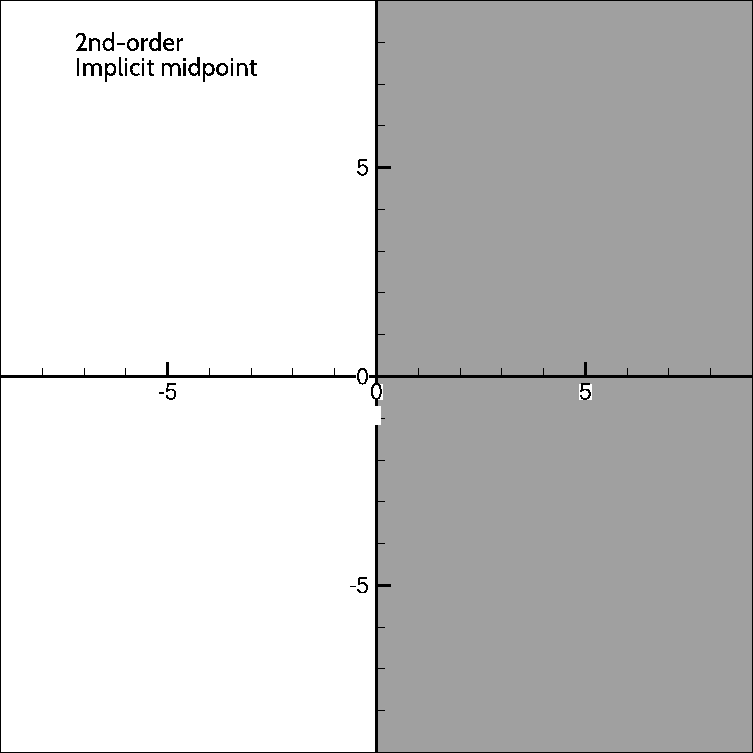
\includegraphics[width=5cm]{2nd.png}};&
				\node[rectangle]{
				  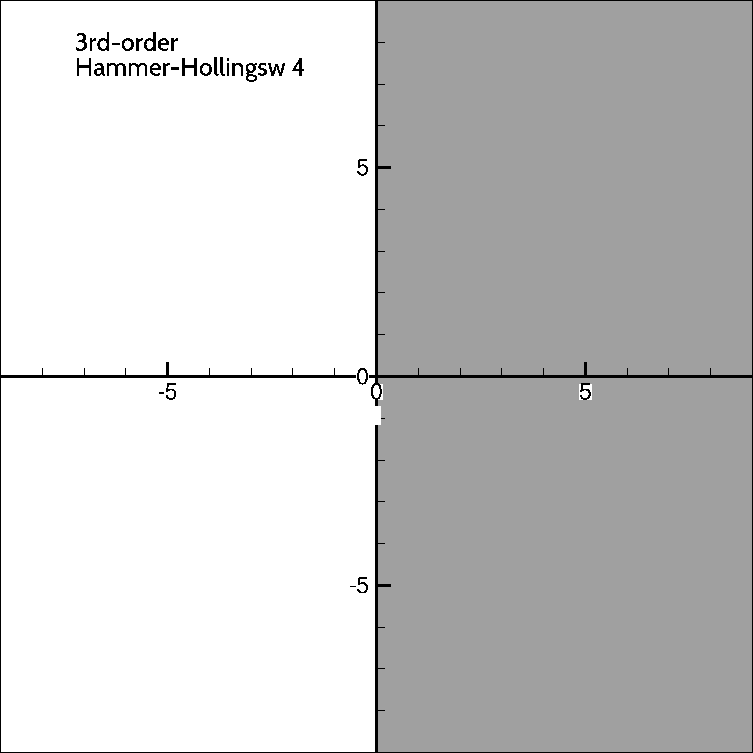
\includegraphics[width=5.cm]{3rd.png}};&
				\node[rectangle]{
	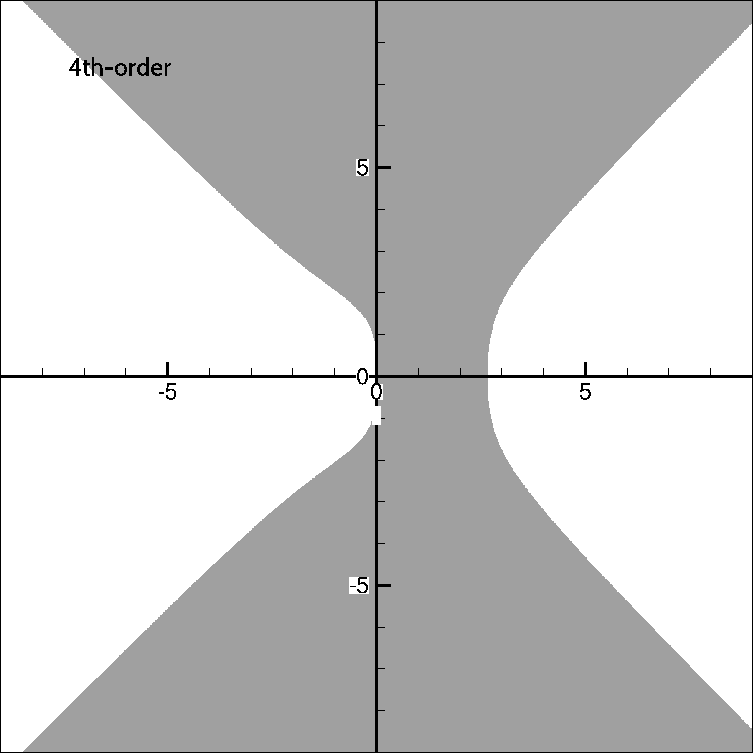
\includegraphics[width=5.cm]{4th.png}};\\
				\node[rectangle]{
				  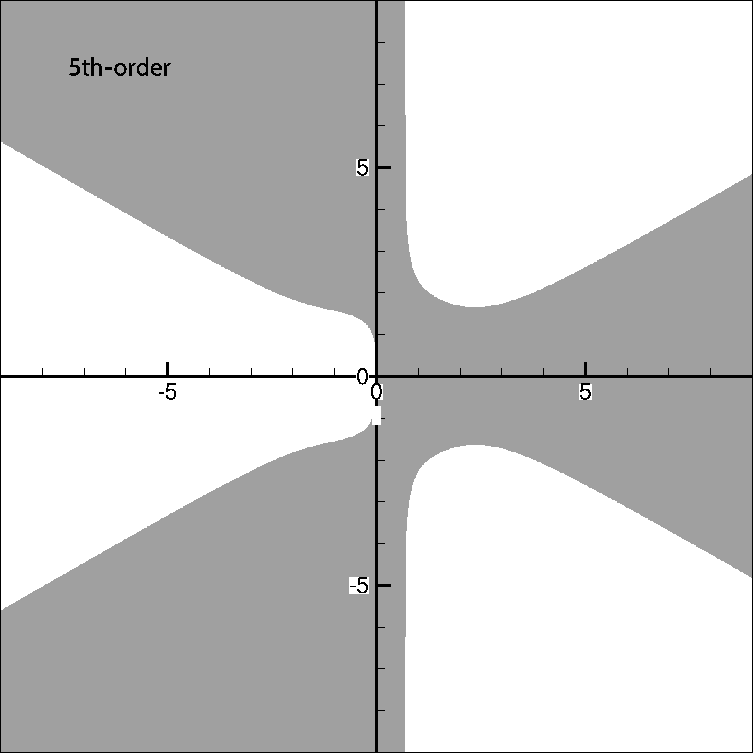
\includegraphics[width=5.cm]{5th.png}};&
				  \node[rectangle]{
					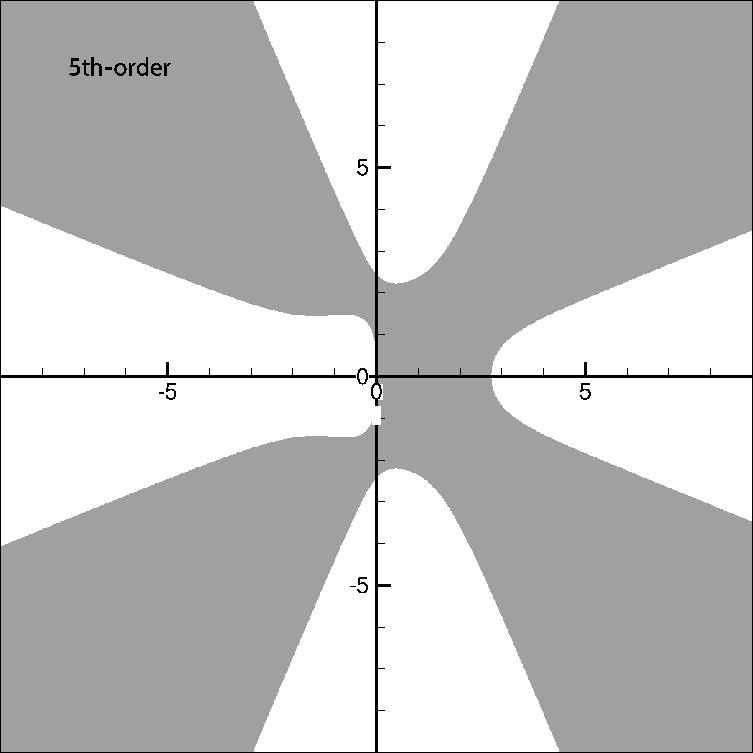
\includegraphics[width=5.cm]{6th.png}};&
				\node[rectangle]{
				  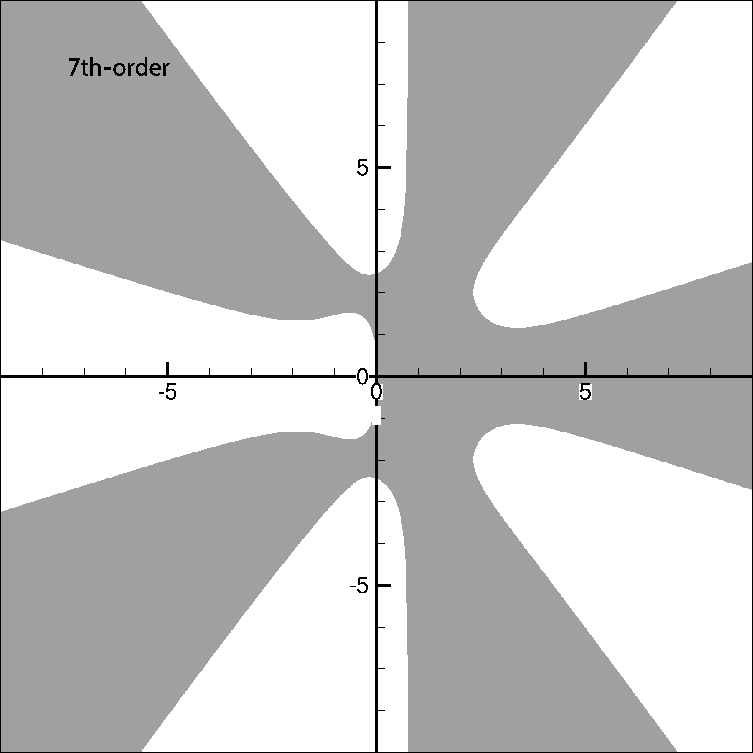
\includegraphics[width=5cm]{7th.png}};\\
				\node[rectangle]{
				  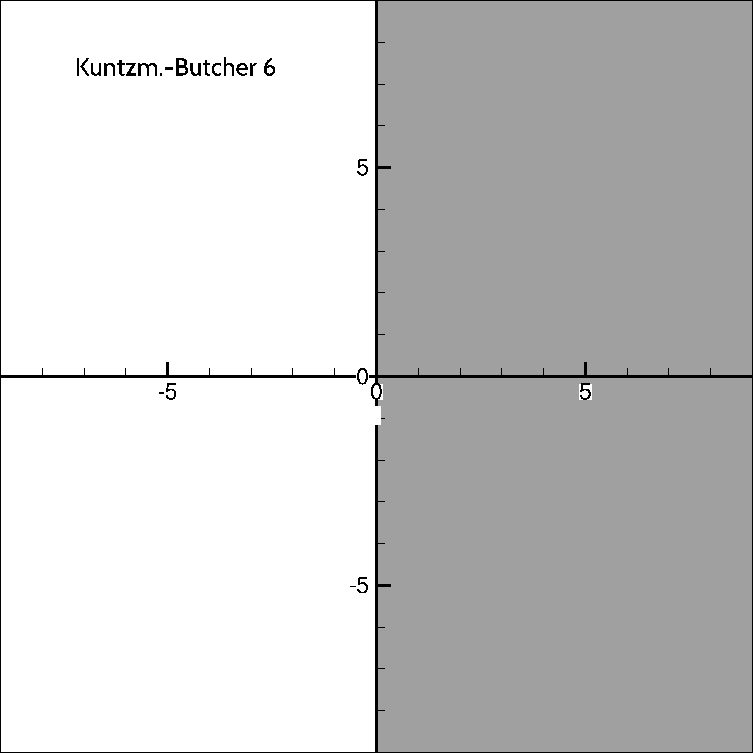
\includegraphics[width=5cm]{Kuntzm6.png}};&
				\node[rectangle]{
				  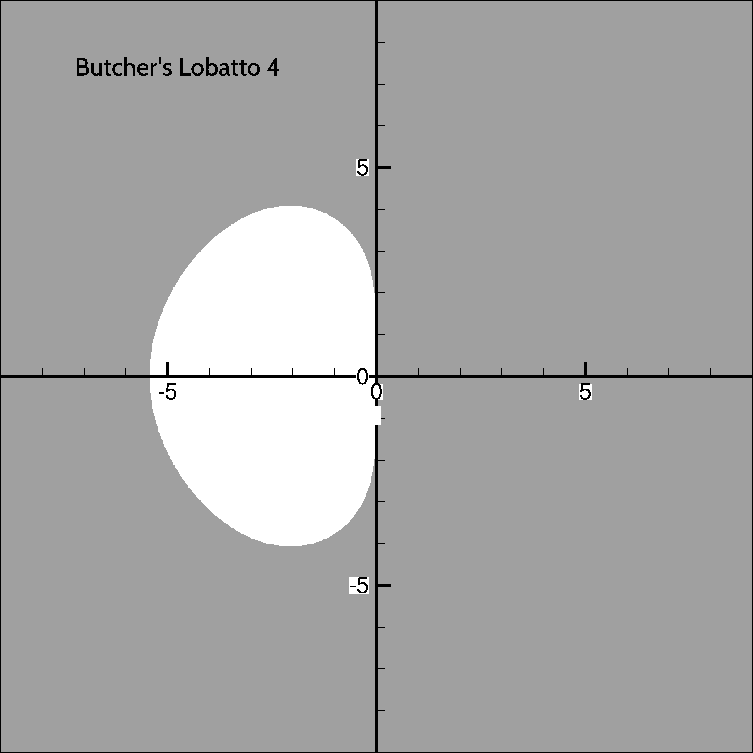
\includegraphics[width=5cm]{Butcher4.png}};&
				\node[rectangle]{
				  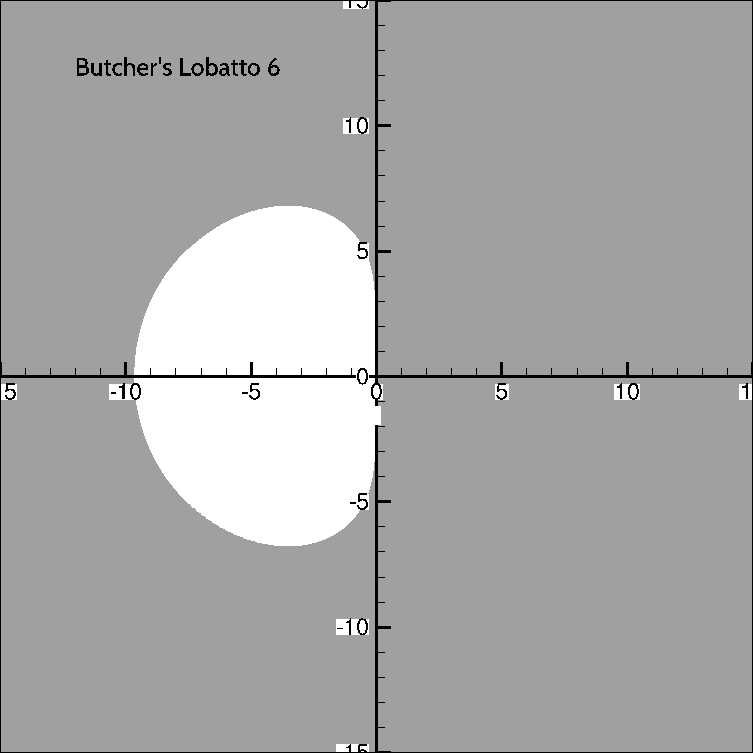
\includegraphics[width=5cm]{Butcher6.png}};\\
		};
	\end{tikzpicture}
	\caption{Stability domains for NP schemes }
	\label{fig1}
\end{figure}
\section{Transformed coefficients NP method}  
Although the NP methods have  the similar stability with the implicit Runge-Kutta methods, but  not all of them can  achieve  A-stability and none of them reaches L-stability. We still hope for a more stable property of NP method.     
A possible way is  to construct a new perturbation term $\overline{p_N}$ by transforming  the coeffients in it.

As $p_N = p + O(\Delta t^{N})$, if $\overline{p_N}= p_N + O(\Delta t^{N})$, the new NP scheme has the same truction error order with the old one. Here, we  assume the new $\overline{p_N}$ with the form
\begin{equation}
  \overline{p_N} = \frac{ 1+ b_1 \Delta t+  b_2\Delta t +\cdots +b_{N-1}\Delta t^{N-1}}{1+c_1\Delta t +c_2\Delta_t^2 +\cdots+ c_{N-2}\Delta t^{N-2}}.
  \end{equation}
and 
  $c_{N-2}=-b_{N-1}/f_y'$.
  Here we have $2N-4$ coeffients and $N-1$ power series relations, so $N-3$ coeffients are  unditermined. In follows, we will consider the transformed  NP method in different orders.    

  \subsection{ The third-order transformed NP method}
The second order method has too little coeffcients, there is no space to  transform, so we begin with the third-order method. For the third-order method with $p_3$, there is no undetermined coefficients,  the new 
\begin{equation}
\overline{p_3} =
\frac{ 1+ b_1 \Delta t+ b_2\Delta t^2}{1+c_1 \Delta t} = 1+a_1\Delta t +a_2 \Delta t^2 + O(\Delta t^3),
\end{equation}
where $c_1=-b_2 /f_y'$. The transformed coeffcients can be solved by the relations
\begin{equation}
  \begin{aligned}
	&b_1=a_1+c_1\\
	&b_2=a_2+a_1c_1\\
	\end{aligned}
\end{equation}

Then the transformed coeffients $b_1$ and $b_2$ are  
\begin{equation}
  b_1= a_1- \frac{a_2}{f_y'+a_1},\hspace{0.3cm}  b_2=\frac{a_2}{1+a_1/f_y'}
\end{equation}

It is easy to get the stability function as 
\begin{equation}
  R(h) = \frac{1+h/3}{1-2h/3+h^2/6}
\end{equation}

\subsection{The fourth-order transformed NP method}
The perturbation term for  the fourth-order NP method is in the  form 
\begin{equation}
  \overline{p_4} = \frac{1+b_1 \Delta t + b_2 \Delta t^2 +b_3\Delta t^3}{1+c_1 \Delta t +c_2 \Delta t^2}
  \end{equation}
  and 
$	c_2= -b_3/f_y'$.
By  the relation 
\begin{equation}
  \overline{p_4}= 1+a_1 \Delta t + a_2\Delta t^2 +a_3\Delta t^3 +O(\Delta t^4).
  \end{equation}
We can get the relations
\begin{equation}
  \begin{aligned}
  b_1= a_1+ c_1\\
  b_2= a_2+a_1c_1 +c_2\\
  b_3= a_3+a_2c_1+a_1c_2\\
  \end{aligned}
  \end{equation}
 In  the 4th-order method the $c_1$ is undetermined, we set  $c_1 = -6a_1$.  Then the transformed coefficients are
 \begin{equation}
   \begin{aligned}
   &c_1=-6a_1,c_2=-b_3/f_y'\\
   &b_1=-5a_1, b_2=a_2-6a_1^2-\frac{a_3-6a_1a_2}{f_y'+a_1}, b_3=\frac{a_3-6a_1a_2}{1+a_1/f_y'}
   \end{aligned}
   \end{equation}
t 
 The stability function is given as 
  \begin{equation}
	R(h)=\frac{1+7h/2+5h^2/4}{1+5h/2-7h^2/4+h^3/3}
	\end{equation}
	\subsection{The fifth-order transformed NP methods}
The perturbation term for the fifth-order NP method is
\begin{equation}
  \overline{p_5} = \frac{1+b_1 \Delta t + b_2 \Delta t^2 +b_3\Delta t^3 +b_4\Delta t^4 }{1+c_1 \Delta t+c_2 \Delta t^2 +c_3 \Delta t^3},
  \end{equation}
  and $c_3=-b_4 /f_y'$.
The transformed coefficients are obtained as follows
\begin{equation}
  \begin{aligned}
  &b_1=a_1+c_1\\
  &b_2=a_2+a_1c_1+c_2\\
  &b_3=a_3+a_2c_1+a_1c_2+c_3\\
  &b_4=a_4+a_3c_1+a_2c_2+a_1c_3\\
  \end{aligned}
 \end{equation}
We set the undetermined coefficients  as $c_1= -6a_1, c_2=-144a_2$. Then the transformed coefficients are get as
\begin{equation}
  \begin{aligned}
	&c_1=-6a_1, c_2=-144a_2, c_3=-b_4/f_y'\\
	&b_1=-5a_1, b_2=-6a_1^2-143a_2,  b_3=a_3-150a_1a_2- \frac{a_4-4a_1a_3+29a_2^2}{f_y'+a_1} ,b_4=\frac{a_4-6a_1a_3-144a_2^2}{1+a_1/f_y'}  \\
	\end{aligned}
	\end{equation}



The stability function is
 \begin{equation}
   R(h)=\frac{1+7h/2-125h^2/12-1229h^3/360}{1+5h/2-161h^2/12+3091h^3/360-871h^4/360}
   \end{equation}
   \subsection{The  sixth-order transformed NP method} 
The perturbation term for the sixth-order NP method is
\begin{equation}
  \overline{p_6} = \frac{1+b_1 \Delta t + b_2 \Delta t^2 +b_3\Delta t^3+b_4\Delta t^4 +b_5 \Delta t^5}{1+c_1 \Delta t +c_2 \Delta t^2+c_3 \Delta t^3 +c_4 \Delta t^4}
  \end{equation}
  and 
$c_4= -b_5/f_y'$
The transformed coefficients are obtained as follows
\begin{equation}
  \begin{aligned}
  &b_1=a_1+c_1\\
  &b_2=a_2+a_1c_1+c_2\\
  &b_3=a_3+a_2c_1+a_1c_2+c_3\\
  &b_4=a_4+a_3c_1+a_2c_2+a_1c_3+c_4\\
  &b_5=a_5+a_4c_1+a_3c_2+a_2c_3+a_1c_4\\
  \end{aligned}
 \end{equation}
We use the undetermined coefficients $c_1=-6a_1,c_2=144a_2$,and $c_3=600a_3$. Then the stability function is
\begin{equation}
  R(h)=\frac{1+7h/2-125h/12-263h^3/6-2029h^4/144}{1+5h/2-161h^2/12-335h^3/6+5171h^4/144-3643h^5/360}
  \end{equation}

	\subsection{The  seven-order transformed NP methods}
\begin{equation}
  \overline{p_7} = \frac{1+b_1 \Delta t + b_2 \Delta t^2 +b_3\Delta t^3 +b_4\Delta t^4  +b_5 \Delta t^5 +b_6\Delta t^6}{1+c_1 \Delta t+c_2 \Delta t^2 +c_3 \Delta t^3+c_4 \Delta t^4 +c_5 \Delta t^5},
  \end{equation}
  and $c_5=-b_6 /f_y'$.
The transformed coefficients are obtained as follows
\begin{equation}
  \begin{aligned}
  &b_1=a_1+c_1\\
  &b_2=a_2+a_1c_1\\
  &b_3=a_3+a_2c_1+a_1c_2+c_3\\
  &b_4=a_4+a_3c_1+a_2c_2+a_1c_3+c_4\\
  &b_5=a_5+a_4c_1+a_3c_2+a_2c_3+a_1c_4+c_5\\
  &b_6=a_6+a_5c_1+a_4c_2+a_3c_3+a_2c_4+a_1c_5\\
  \end{aligned}
 \end{equation}
The undetermined coefficients are set as  $c_1=-6a_1,c_2=144a_2, c_3=-144a_3$ and $c_4=1440a_4$. The stability function is 
\begin{equation}
  R(h)=
  \frac{1+7h/2+163h^2/12+109h^3/6+39449h^4/720+52063h^5/3024}{1+5h/2+127h^2/12+37h^3/6+30809h^4/720-15207h^5/494+52091h^6/7560}
\end{equation}
\section{The stability analysis of the transformed NP method}
The stability functions  of the transformed NP methods are  collected in Table \ref{tab:2}, and the stablility domains are showed in Fig.\ref{fig2}.  It is  obviously that all the 3rd-order to 7th-order transformed NP methods are A-stable and L-stable and their unstability domains are limited in finite regions.



\begin{table}[htbp]
  \small 
  \centering
  \setlength{\belowcaptionskip}{10pt}
  \caption{\small The stable functions of N-th order transformed  NP methods} 
  \begin{tabular}{ll}
	\toprule
Order & $R(h)$\\
\midrule
3 & $\frac{1+h/3}{1-2h/3+h^2/6}$\\
4& $\frac{1+7h/2+5h^2/4}{1+5h/2-7h^2/4+h^3/3}$\\
5 & $\frac{1+7h/2-125h^2/12-1229h^3/360}{1+5h/2-161h^2/12+3091h^3/360-871h^4/360}$\\
6& $\frac{1+7h/2-125h/12-263h^3/6-2029h^4/144}{1+5h/2-161h^2/12-335h^3/6+5171h^4/144-3643h^5/360}$\\
7 & $
  \frac{1+7h/2+163h^2/12+109h^3/6+39449h^4/720+52063h^5/3024}{1+5h/2+127h^2/12+37h^3/6+30809h^4/720-15207h^5/494+52091h^6/7560}$\\
  \bottomrule
\end{tabular}\label{tab:2}
\end{table}


\begin{figure}
  \centering
				  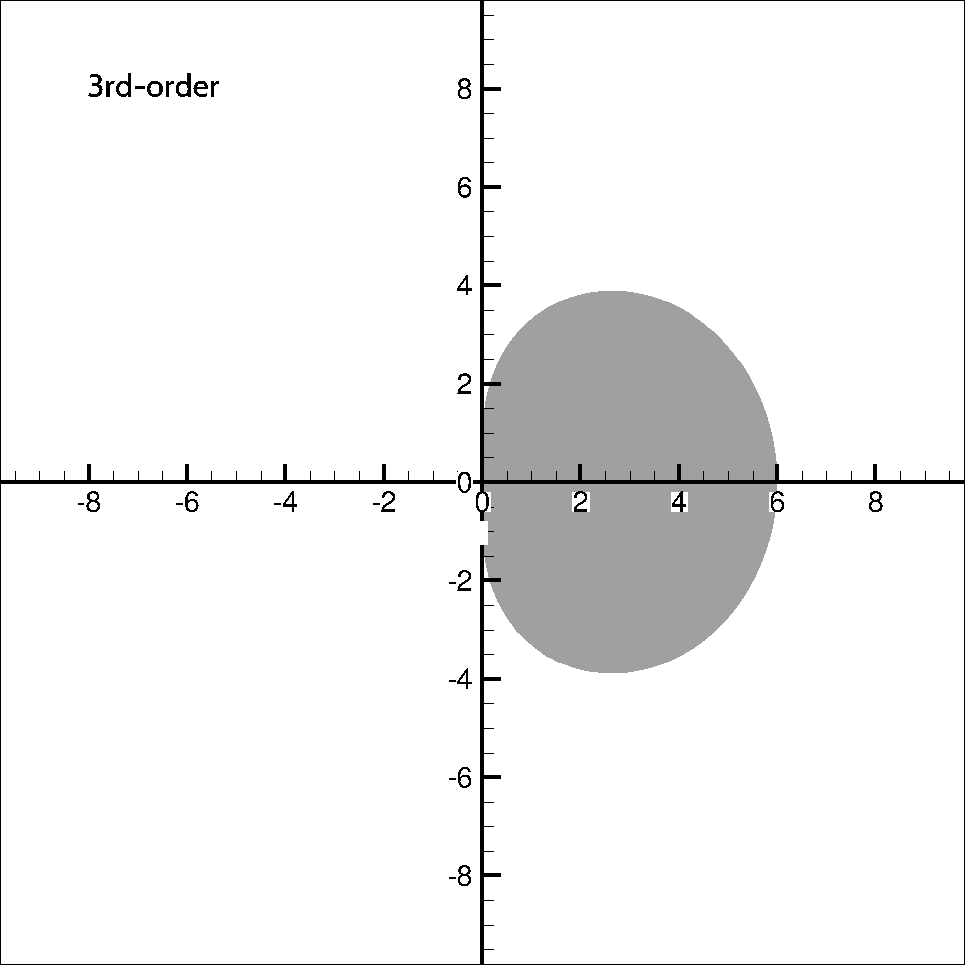
\includegraphics[width=5cm]{3rd_tran.png}
				  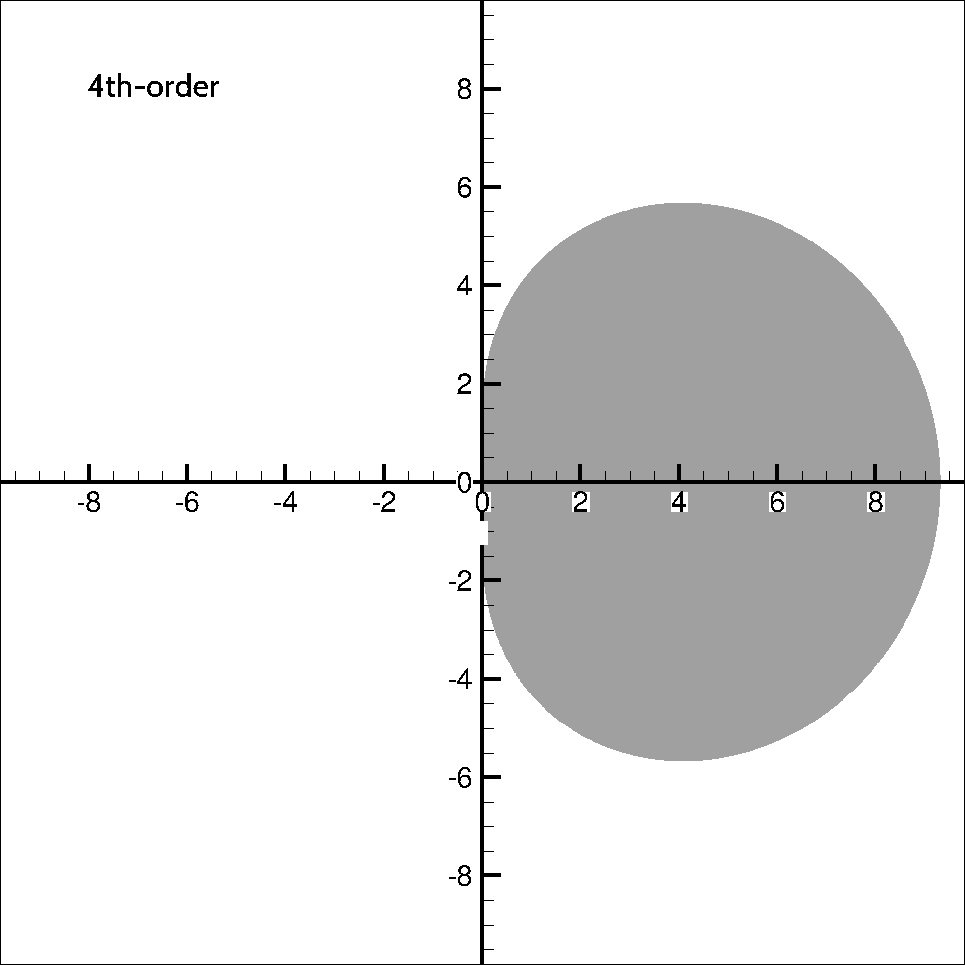
\includegraphics[width=5.cm]{4th_tran.png}
					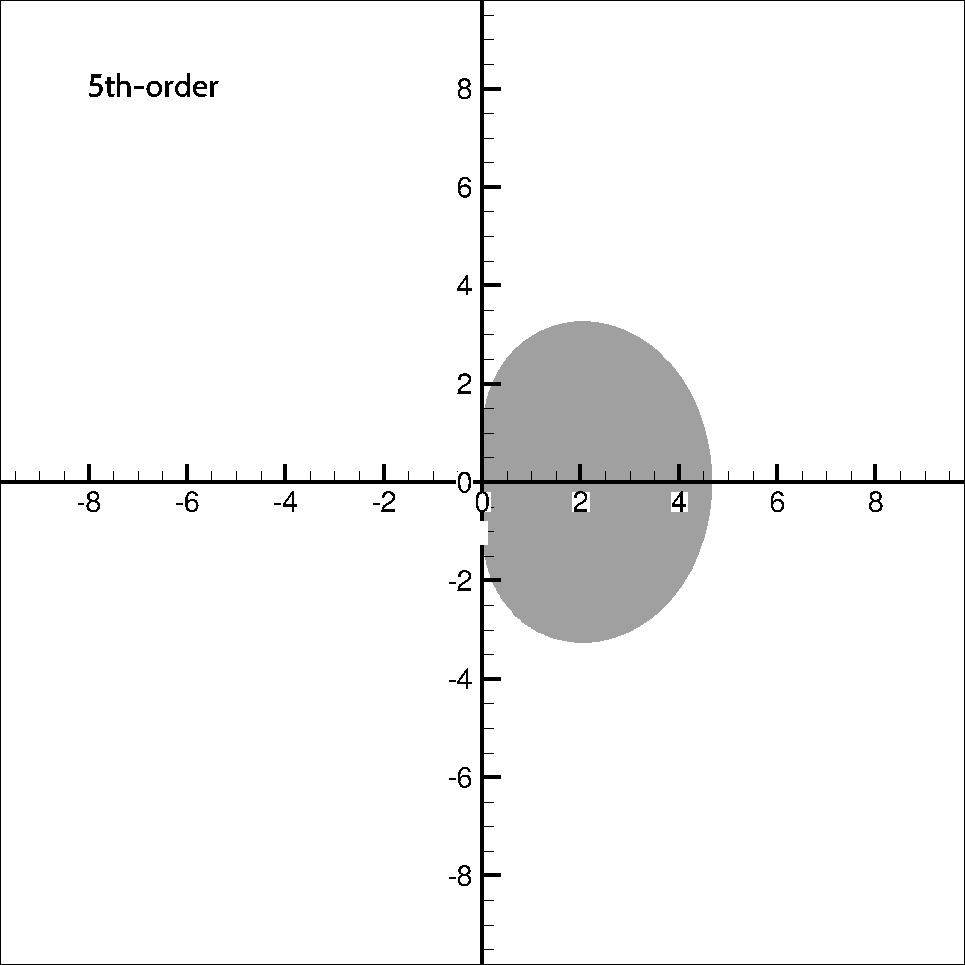
\includegraphics[width=5.cm]{5th_tran.png}}

					\centering
				  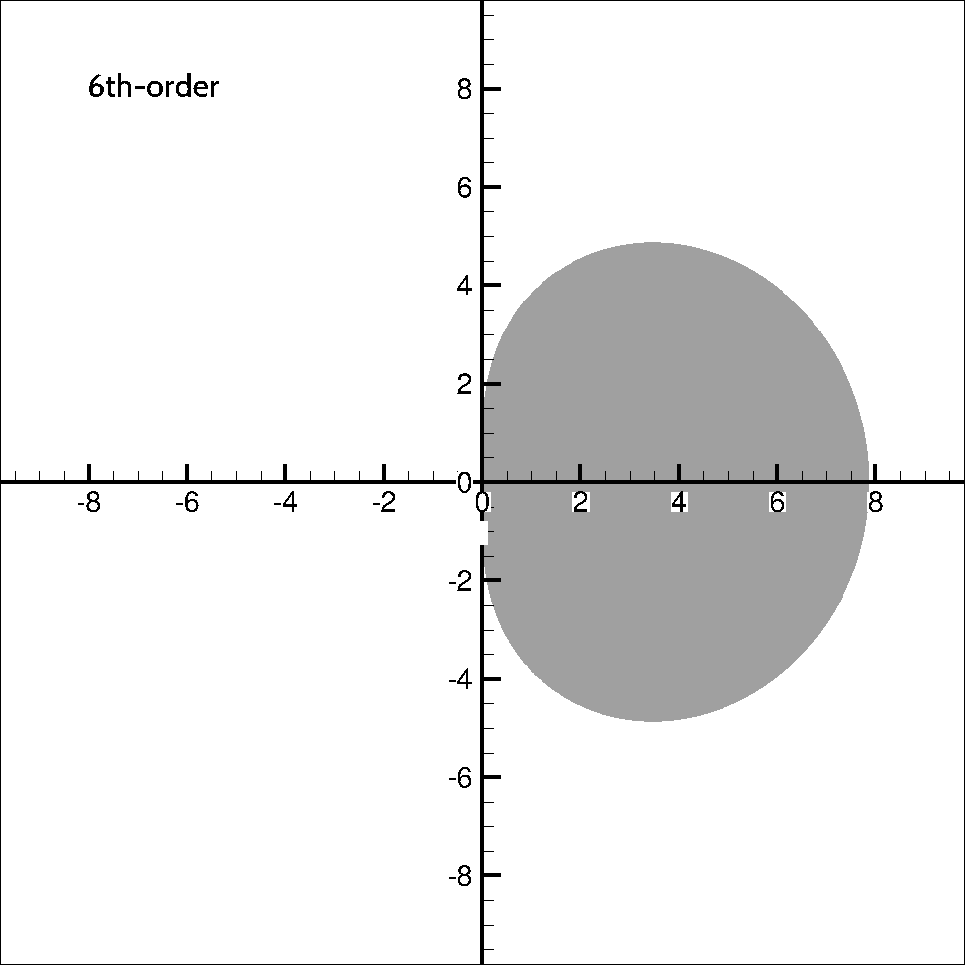
\includegraphics[width=5.cm]{6th_tran.png}
				  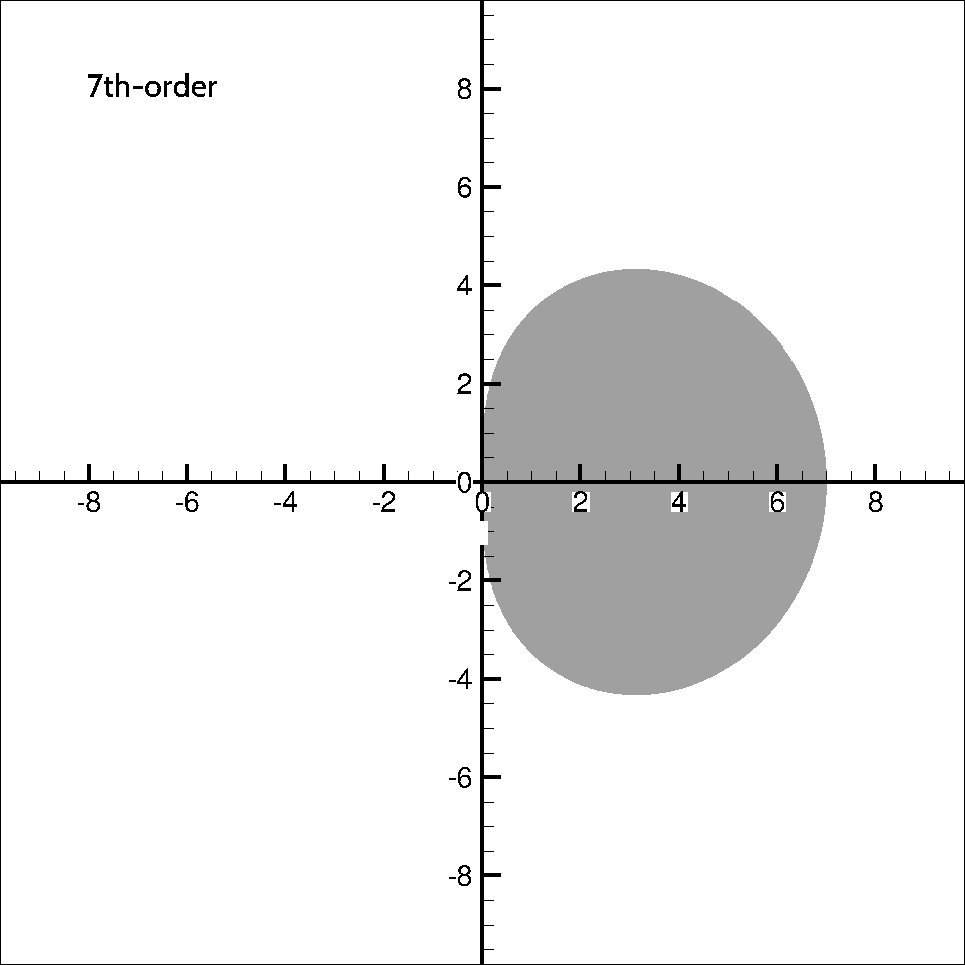
\includegraphics[width=5cm]{7th_tran.png}
	\caption{Stability domains for the transformed NP methods }
	\label{fig2}
\end{figure}


\section{Numerical tests for the NP methods and the transformed NP methods}
Some numerical tests are considered in this section. There are two purposes, one is to show the construction process of the NP methods in  the real coding and using background as the new methods are far from the methods frequently used; the other one purpose is to test the real performance of the new method espcially in the  computing of the nolinear ODE and ODEs.

Example 1 \cite{Seinfeld1970Review,Prothero1974On}

\begin{equation} \label{eq:3}
  \begin{aligned}
	&y'(x)=g'(x)+\lambda (y-g(x)), \hspace{0.3cm} y=g(0) \hspace{0.1cm}  \text{at} \hspace{0.1cm} x=0\\
	&g(x)=10-(10+x)e^{-x},  \hspace{0.3cm} \lambda \hspace{0.1cm} \text{real}.
  \end{aligned}
  \end{equation}

  In this example we consider the order changing  with different stiffness which determined  by $\Delta x \lambda$. For the method without stiff stability, the order will drop significantly when $\Delta x \lambda$ is large. 

  For Eq.(\ref{eq:3}) the high-order derivatives are
\begin{equation}
  y^{(n)}=g^{(n)}+\lambda (y^{(n-1)}-g^{(n-1)}) , \hspace{0.3cm} n=2,3,\cdots
  y'=(9+x)e^{-x}+\lambda [y-10+(10+x)]e^{-x}\\
  y''=(9+x)e^{-x}+\lambda [y-10+(10+x)]e^{-x}\\
\end{equation}
and
\begin{equation}
  \begin{aligned}
  &g'=(9+x)e^{-x},
  g''=-(8+x)e^{-x},
  g^{(3)}=(7+x)e^{-x}\\
  &g^{(4)}=-(6+x)e^{-x},
  g^{(5)}=(5+x)e^{-x},
  g^{(6)}=-(4+x)e^{-x}.\\
  \end{aligned}
  \end{equation}










\begin{equation}
 \frac{ 1+ b_1 \Delta t+ b_2\Delta t}{1-b_2 \Delta t}= 1+a_1 \Delta t +a_2\Delta t^2 +O(\Delta t^3)
  \end{equation}










  \subsection{The Taylor series method}

  \begin{equation}
	y_{n+1} = y_n + \frac{dy}{dt}\Delta t +\frac{1}{2} \frac{d^2y}{dt^2}+\cdots
	\end{equation}

\begin{equation}
\begin{align}
  f= Ay\\
  \frac{dy}{dt}=f=Ay\\
  \frac{d^2y}{dt^2}= A^2y 
\end{align}
  \end{equation}


  \begin{equation}
	y_{n+1} = y_n + A y_n \Delta t + A^2\Delta t \frac{1}{2} \frac{d^2y}{dt^2}+\cdots
	\end{equation}


 In this paper, we try to develop a high-order stiff-stable explicit numerical method 

This paper is organized as follows. In section 2, we briefly introduce the decoupling method for solving the reactive Euler equations. In section 3, a dual information preserving method is proposed to solve the convection step of species mass fraction equations. In section 4, a numerical perturbation method is developed to solve the fractionated reaction step, analysis of stability and numerical examples are also presented. A series of examples, including one- and two- dimensional problems, simplified reaction model and multi-species reaction models, are given to validate the accuracy and robustness of the new method in section 5. Conclusions are shown in section 6.
This equations is easy to solve for  


\section{Numerical perturbation method}

For Eq(\ref{eq:ode}), one of  the simplest scheme is the first-order explcit Euler scheme  
\begin{equation}\label{eq:euler}
  \bm{y}_{n+1}- \bm{y}_n = \Delta t f(t,\bm{y})
\end{equation}
If we want to improve the accuracy order of scheme (\ref{eq:euler}),  one common method is add 

But as proved by  

A common way to get higher-order accuracy it to use sub-timestep in the intercal $[t,t+\Delta t]$,    with the stable property in an explicit scheme  is to construct unlinear schemes with more derivative informations from the original differential equation (\ref{eq:ode}) 

First, more dericative information can be get from the original differential equation (\ref{eq:ode}) theoretically 








   



\section{Conclusions}

The dual information preserving method is firstly proposed to cure the numerical stiff problem generated in simulating the reacting flows. First, the species mass fraction equations are decoupled from the reactive Euler equations, and then they are further fractionated into the convection step and reaction step. The DIP method is actually proposed to deal with the species convection step. Two kinds of virtual Lagrangian point are introduced, one is limited in each Eulerian cell, and another one is tracked in the whole computation domain. The number of each kind of virtual point is the same as the cell (grid) number.The DIP method can effectively eliminate the spurious propagation speed caused by the intermediate state generated by the numerical dissipation.

In this paper, the numerical perturbation (NP) methods are also developed to solve the fractionated reaction step (ODE equations). The NP schemes show several advantages, such as no iteration, high order accuracy and large stable region.  

A series of numerical examples are used to demonstrate the reliability and robustness of the new methods.

%^The key idea of this method is
%^
%^(1) the particle information, including the current cell number (particle moved in), relative location
%^to the centre of current cell, and the species mass fraction on the point, is calculated and
%^stored. While the cell information only record the position to the cell centre 
%^and the species mass fraction of the cell.  
%^
%^(2) For a fixed cell, if there are information points in it, its information is
%^updated by averaging all paticle points’ information; otherwise, the cell’s information
%^is updated by averaging all entered cell points’ information. If there is none of above
%^two points in a cell, its relative location of the cell point is set to zero and the species mass on it are obtained by interpolating those of contiguous cells. 
%^
%By the new method, the correct activate position of the reaction will be captured even with a course mesh as eliminating the dissapation in the species mass fraction equations. The DIP method is easily extended to multiple reaction models and multi-dimensional problems. Through decoupling process, this method can combine with high order methods for Euler equations system, conveniently. In this paper, numerical perturbation method is also developed to solve the fractioned reaction step (ODE equations) to improve the stability and efficiency. A series of numerical examples are used to test the reliability and robustness of the new methods.  
%In the furture, the DIP method may also be used in traditional interface(surface) problems and reaction flows with more complex reaction models.
%


%In addition, a numerical perturbation method to solve the fractioned reaction step (ODE equation) to improve the stability and
%efficiency.





%we developed a series of high-order numerical perturbation method for stiff ODE equations and Dual Information Preserving(DIP) method for mass fraction convection equations to capture the reaction interface. Combine them and use a new decoupling method we gave a solving system for reactive Euler equations with high order. We can cure the difficulty in numerical simulations of the conservation equations with stiff source terms by the new solving system.  

%With a decoupling method we decouple reactive Euler equations into two parts---Euler equations and mass fraction convection/reaction equations, Euler equations can be solved by fifth-order WENO/third-order Runge-Kutta schemes with a Lax-Friedrichs splitting. Then using fraction step method, we split mass fraction equations into two steps: convection step and reaction step. Third-order transformed perturbation(TP) method is used in solving reaction step ODE equations which is proved to be strong A-stable. Convection step is solved by Dual Information Preserving(DIP) method which uses Lagrangian points based on fixed mesh. Eliminating unphysical smooth in the mass fraction discontinuous caused by the dissipation of spatial difference schemes in convection step, the wrong activation of reaction will not happened. Through a lot numerical examples, includes scalar problems and reactive Euler problems, one- and two- dimension detonation problems, single reaction models and multiple reaction models, the availability and robustness of the new method is tested.

\section*{Acknowledgement} 
This research work was supported by NSFC 11272324, 11272325, NSAF U1530145 and 2016YFA0401200.

\section*{References}

\bibliography{mybibfile}

\end{document}






\end{note}


